\subsection{Programación dinámica}
La programación dinámica es un método de diseño de algoritmos que se puede usar cuando la solución del 
problema se puede ver como el resultado de una sucesión de decisiones. Técnica que se usa principalmente en
problemas de optimización, la cual es por fases en vez de simultánea.
Proporciona un procedimiento sistemático para encontrar la combinación de decisiones que maximice la efectividad
total, al descomponer el problema en etapas, todas ellas enlazadas mediante algoritmos recursivos.



\subsubsection{Origen}
Esta forma de proceder fue inventada por Richard Bellman para optimizar problemas complejos que pueden ser 
secuencializados. La solución de problemas mediante esta técnica se basa en el llamado principio de óptimo enunciado por 
Bellman en 1957 y que dice:
\begin{center}
    \emph{ $"$ En una secuencia de decisiones óptima toda subsecuencia ha de ser también óptima."}
\end{center}

Este principio aunque parece evidente no siempre se puede aplicar, luego es necesario verificar que se cumple para el problema
que estamos tratando. Para que un problema pueda ser abordado por esta técnica ha de cumplir dos condiciones:
\begin{itemize}
    \item La solución debe ser alcanzada a través de una secuencia de decisiones, una en cada etapa.
    \item Dicha secuencia ha de cumplir el principio de óptimo.
\end{itemize}

\begin{figure}[h]
    \centering
    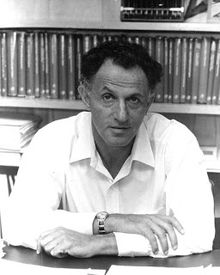
\includegraphics[scale=0.85]{bellman.jpg}
    \caption{Retrato de Richard Bellman.}
\end{figure}

\subsubsection{Características}
En líneas generales un algoritmo de Programación Dinámica se aplica en cuatro fases:
\begin{itemize}
    \item Naturaleza n-etápica del problema.
    \item Verificación del Problema de Optimalidad.
    \item Planteamiento de una recurrencia.
    \item Cálculo de la solución(enfoque adelantado o retardado). 
\end{itemize}

Así que luego comprobaremos que nuestro algoritmo implementado para dar solución al problema de esta práctica es un algoritmo
de Programación Dinámica, viendo que verifica estas cuatro fases.

\subsection{Objetivos}
\begin{itemize}
    \item Conocer qué es la programación dinámica.
    \item Saber determinar si un algoritmo es de programación dinámica.
    \item Ser capaces de implementar un algoritmo de programación dinámica.
\end{itemize}

